\label{sec:5.4}

%%%%%%%%%%%%%%%%%%%%%%%%%%%%%%%%%%%%%%%%%%%%%%%%%%%%%%%
%(Prakash) Discuss SHA/MUX linearity
%%%%%%%%%%%%%%%%%%%%%%%%%%%%%%%%%%%%%%%%%%%%%%%%%%%%%%%

The input signals are sampled at a rate of 2 MS/s, multiplexed by 8 and digitized by one of two calibrated 12-bit pipelined ADCs operating at 16 MS/s. The overall integral non-linearity of the ADC is due to the integral non-linearity of the front-end (SDC), SHA, MUX as well as the overall integral non-linearity in the ADC transfer function. Programming the ColdADC in ADC only mode, frozen SHA mode and free running SHA mode, we were able to measure linearity for ADC only, ADC $+$ SHA and ADC $+$ SHA $+$ MUX configurations. 
%The linearity of the ADC is approximately reduced by 0.3 LSB when SHA is in free running mode, i.e ADC $+$ SHA $+$ MUX. We did not observe any noticeable degradation of linearity between ADC only and frozen SHA mode. However, 

During the frozen SHA mode (ADC $+$ SHA) we observed that overall linearity is slightly different for different sample sets. In this mode, the ADC will oversample the SHA output by a factor of 8 and the linearity of the ADC can be calculated by taking any of the samples. Figure \ref{fig:sha_sample_hist} show that the samples are not consistent and non-linearity has been introduced by SHA/MUX combination. The main source of non-linearity could be SHA op-amps or the MUX.
%Studies were performed at two configuration settings, forzen SHA mode and free running SHA mode. Nominal operation is free running SHA mode. 
\begin{figure}[h!]
\centering
  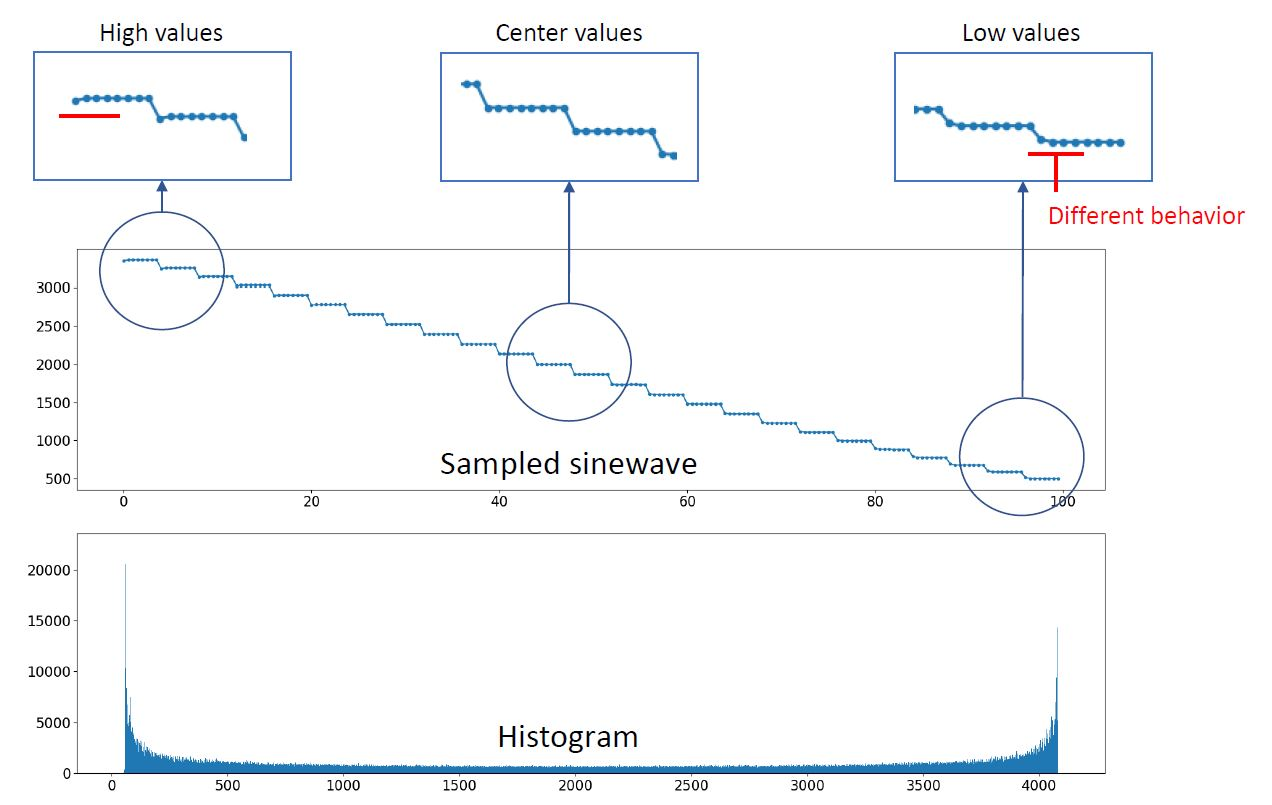
\includegraphics[width=0.7\linewidth]{figures/prakash_fig/sha_sample_hist.JPG}
  \caption{Histogram of ADC sampling in frozen SHA configuration}
  \label{fig:sha_sample_hist}
\end{figure}

To narrow down if any of this non-linearity was causing by the SHA op-amps, we varied the SHA bias current. The change in the SHA bias current did not affect the overall linearity of the ADC, and therefore, we were able to rule out SHA op-amps as the source of non-linearity. Figure~\ref{fig:linearity_sha_current} shows the linearity of ADC measured by looking at the second sample of channel 7 at 40$\mu$A, 50$\mu$A (default) and 60$\mu$A SHA bias currents. These measurements were taken at room temperature with nominal sample rate. 
\begin{figure}[h!]
\centering
  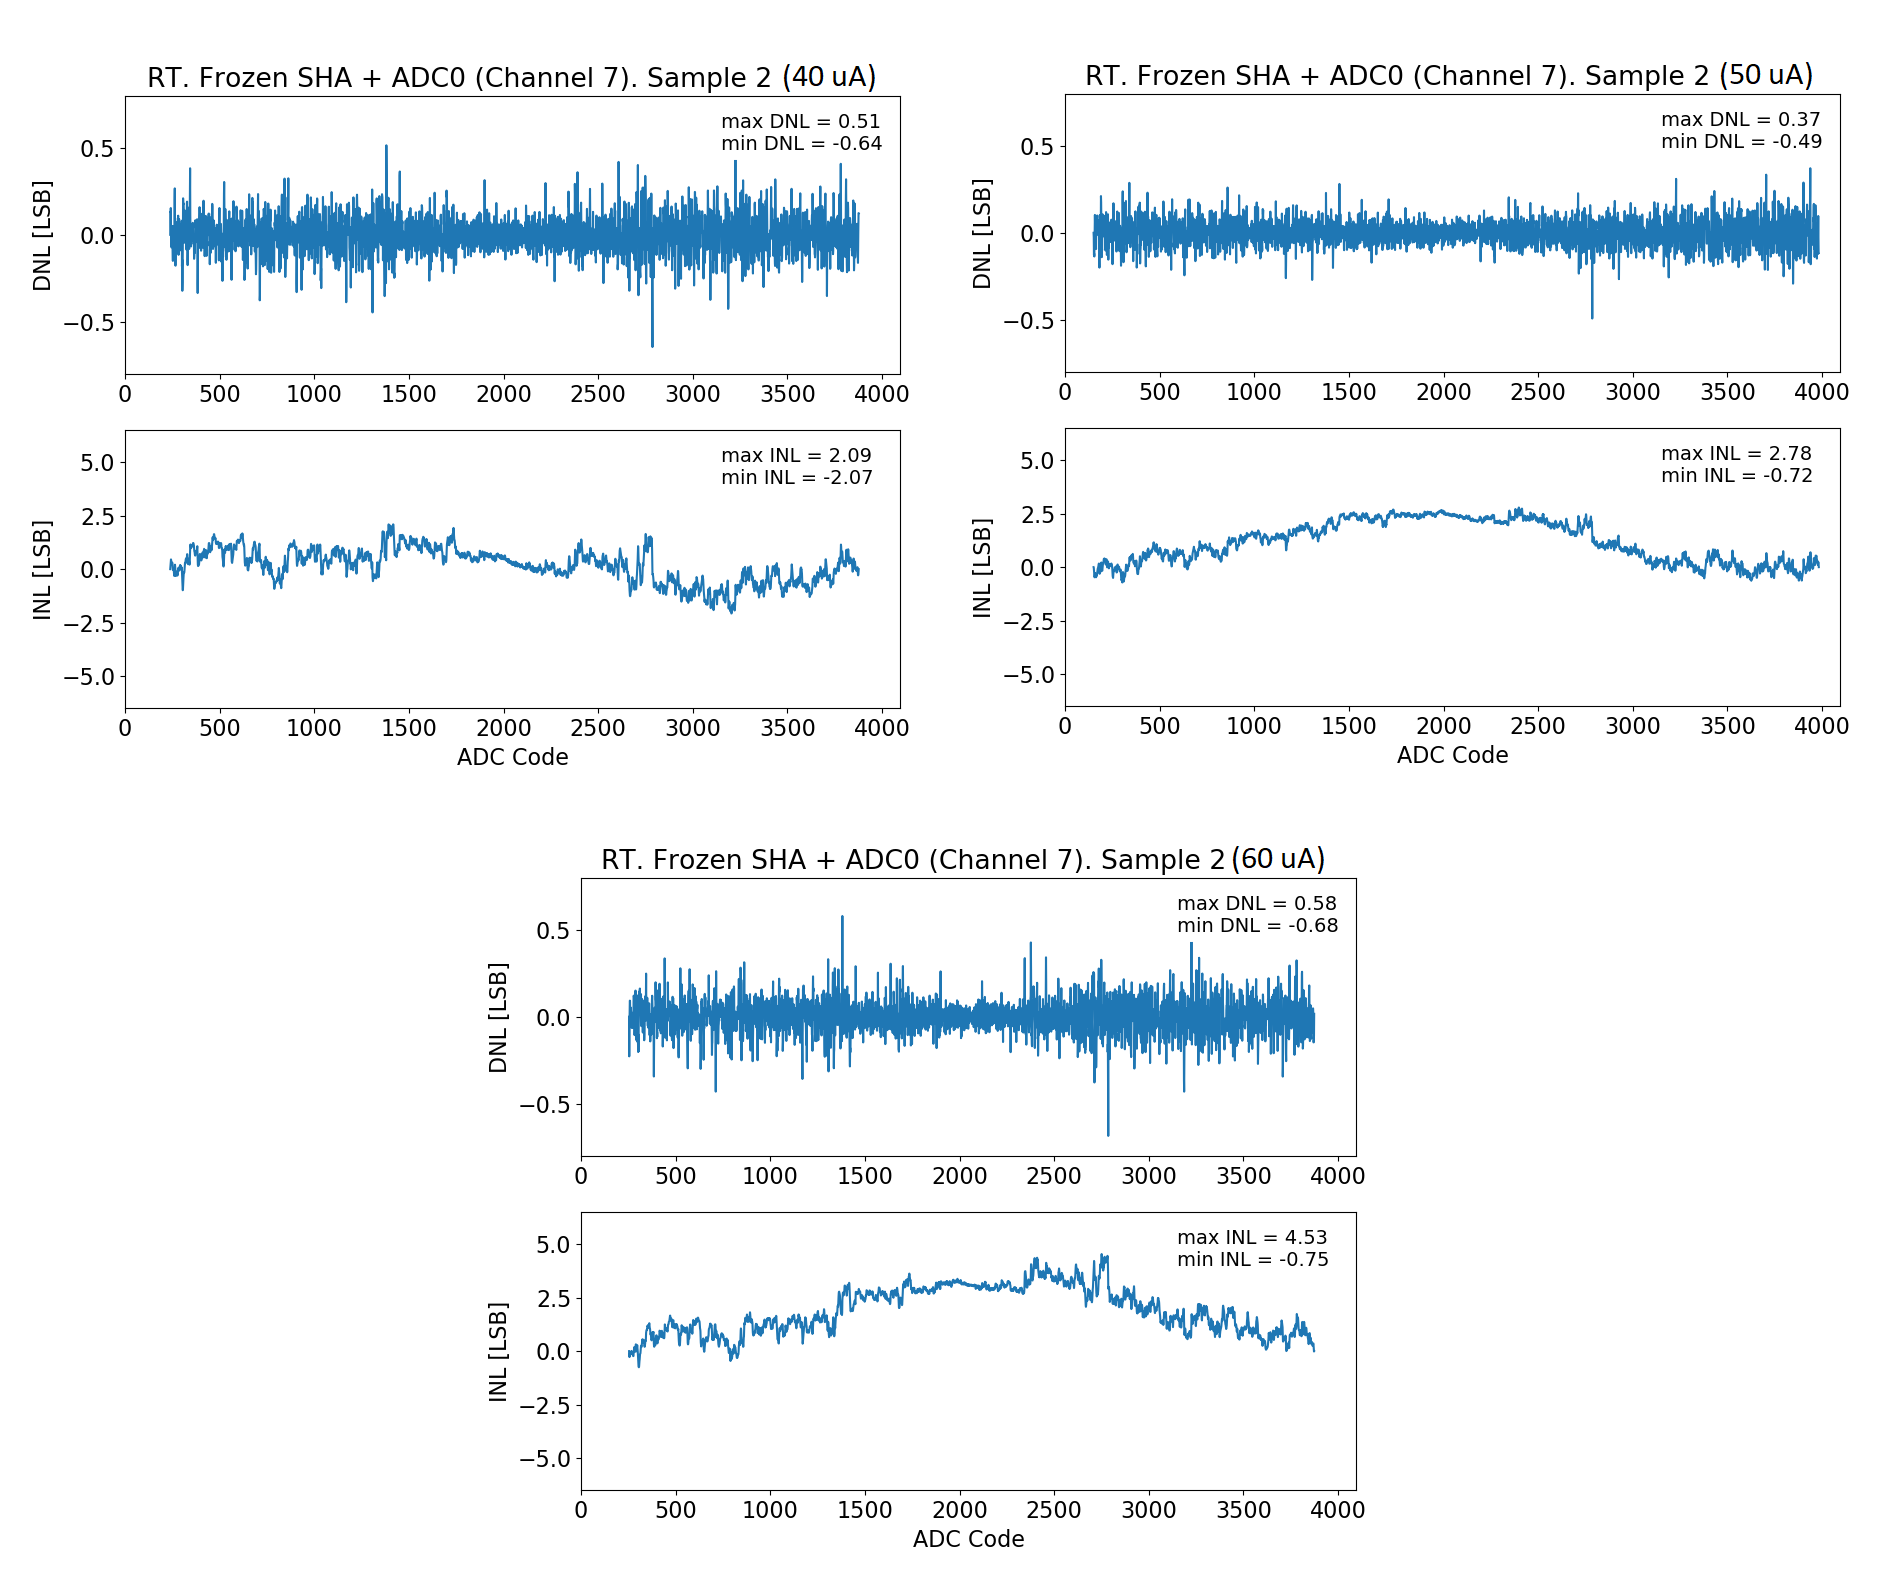
\includegraphics[width=1.0\linewidth]{figures/prakash_fig/linearity_sha_current.png}
  \caption{Linearity of ADC at room temperature with SHA bias current configured to 40, 50, and 60 $\mu$A.}
  \label{fig:linearity_sha_current}
\end{figure}

For our next experiment, we reduced the sampling speed of the ADC. With reduced sampling speed the MUX's will have more time to settle and there will not be any kickback. Figure~\ref{fig:linearity_mux_speed} shows the overall linearity at different sampling clocks. Reducing the sampling frequency improves the linearity significantly. The MUX's seem to be causing the non-linearity and we believe the kickback is the main source of the problem. To address this problem we plan to redesign the MUX to be much faster.
\begin{figure}[h!]
\centering
  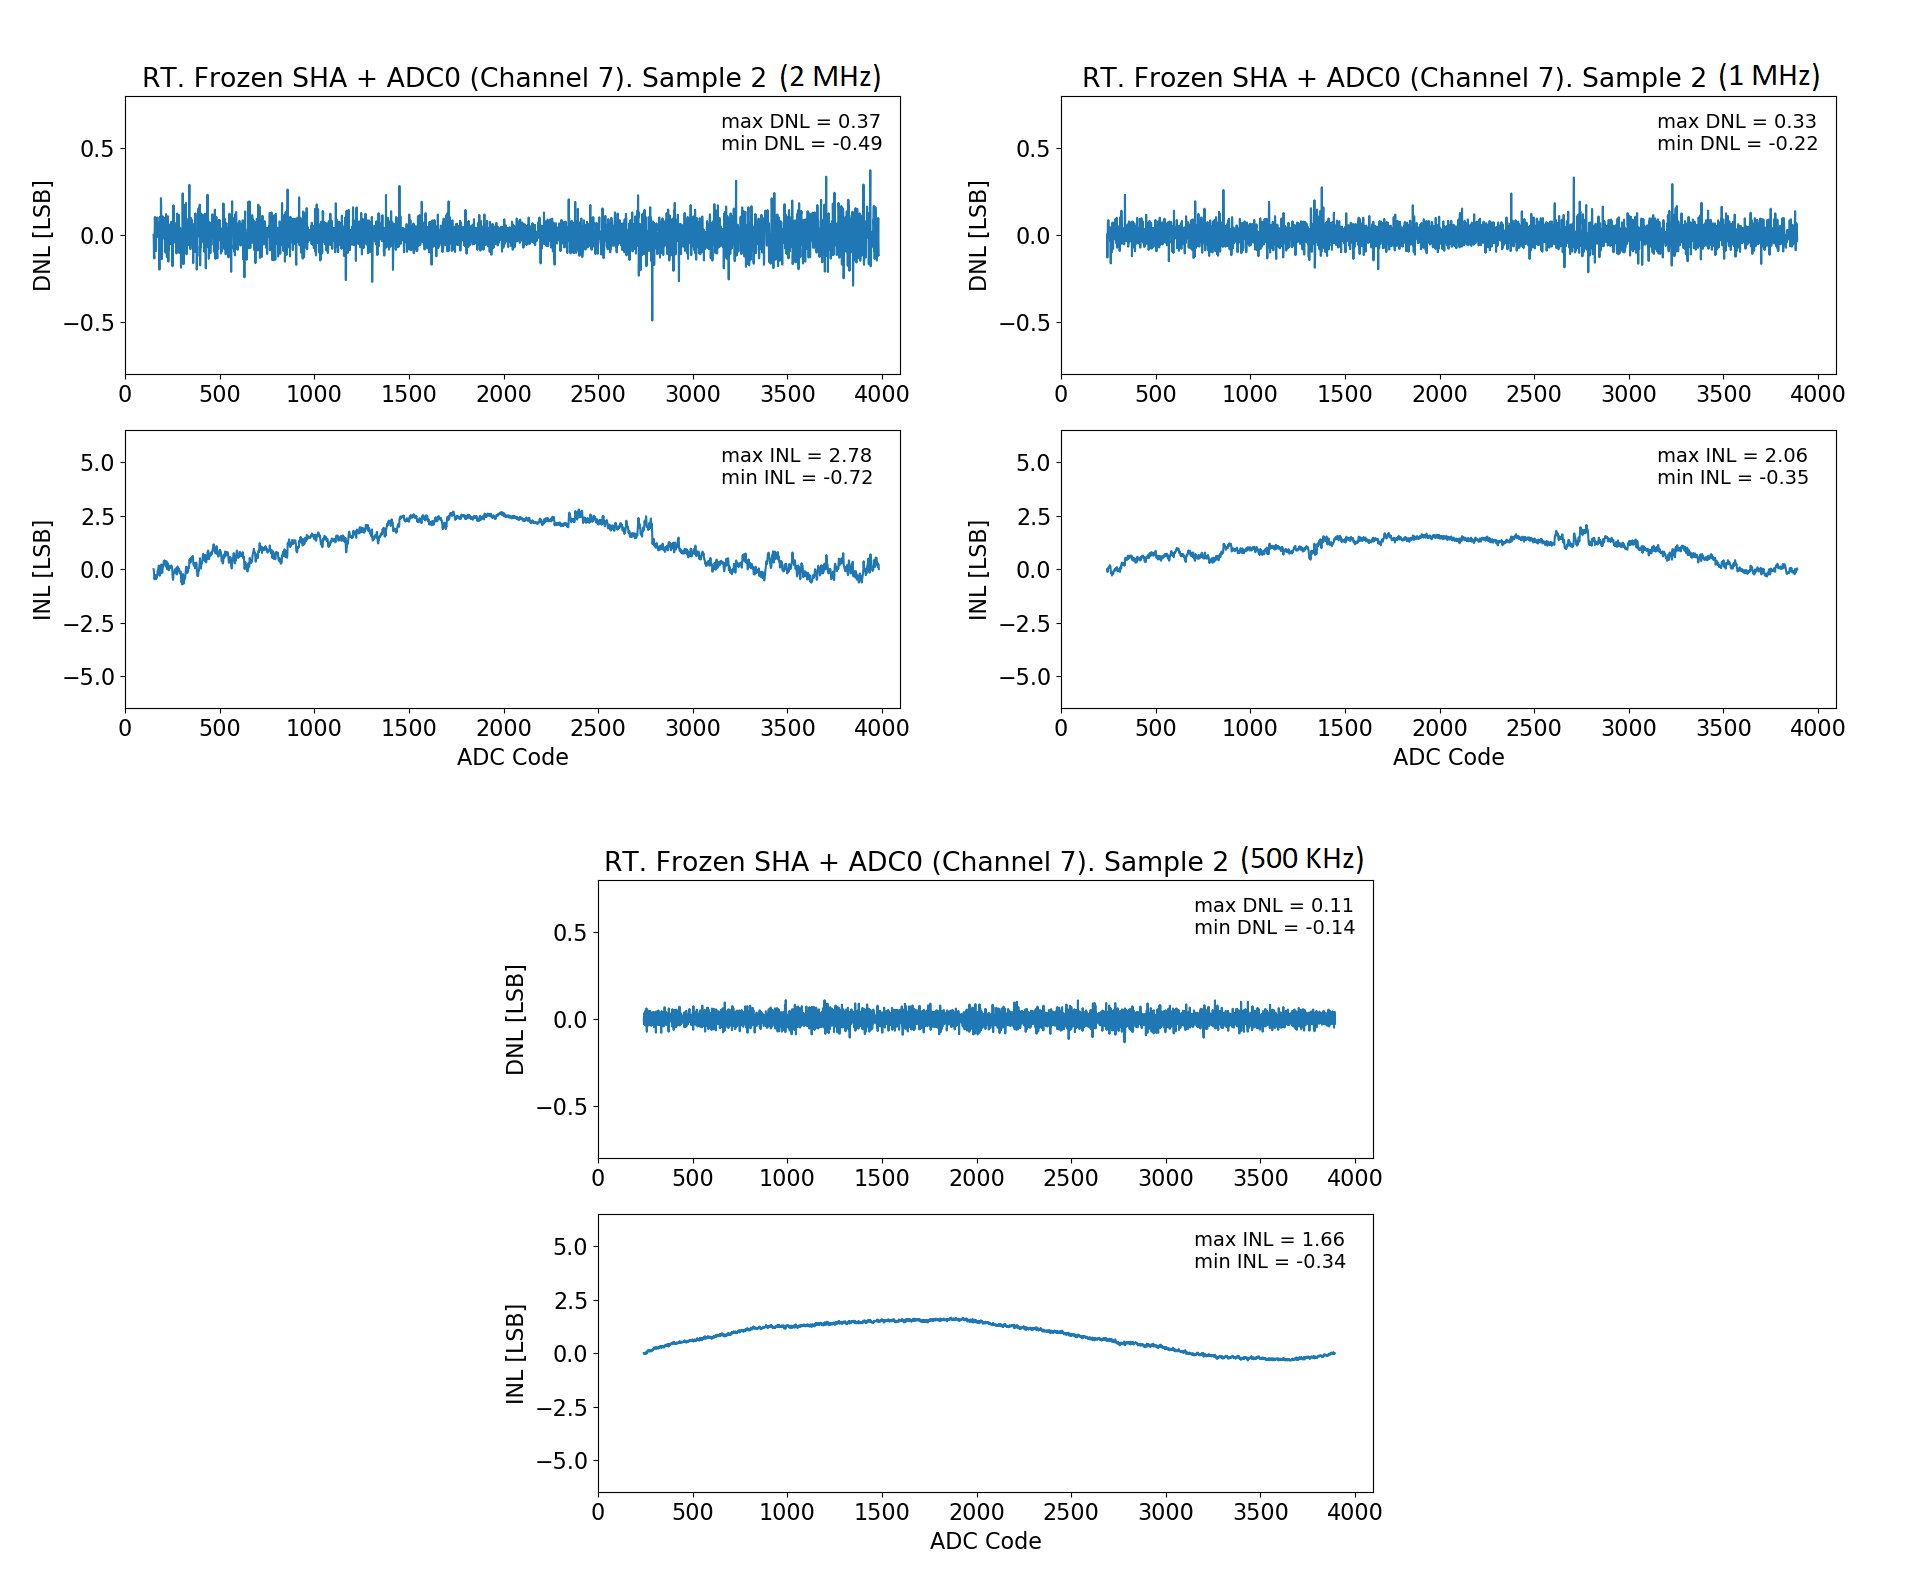
\includegraphics[width=1.0\linewidth]{figures/prakash_fig/linearity_mux_speed.png}
  \caption{Linearity of ADC at room temperature with 2, 1, 0.5 MHz sampling frequencies.}
  \label{fig:linearity_mux_speed}
\end{figure}

During the frozen SHA configuration, we observed overall linearity improvement compared to free running SHA configuration. Figure \ref{fig:linearity_rt_free_frozen} shows the difference in linearity between free running SHA and frozen SHA at room temperature. The improvement in linearity can be attributed to the MUX's not being clocked in the frozen SHA mode. Redesign of MUX is necessary to improve the linearity of the ADC in the free running SHA mode. 
%By redesigning the MUX's to be faster we can improve the linearity of the ADC in the free running SHA mode. 
\begin{figure}[h!]
\centering
  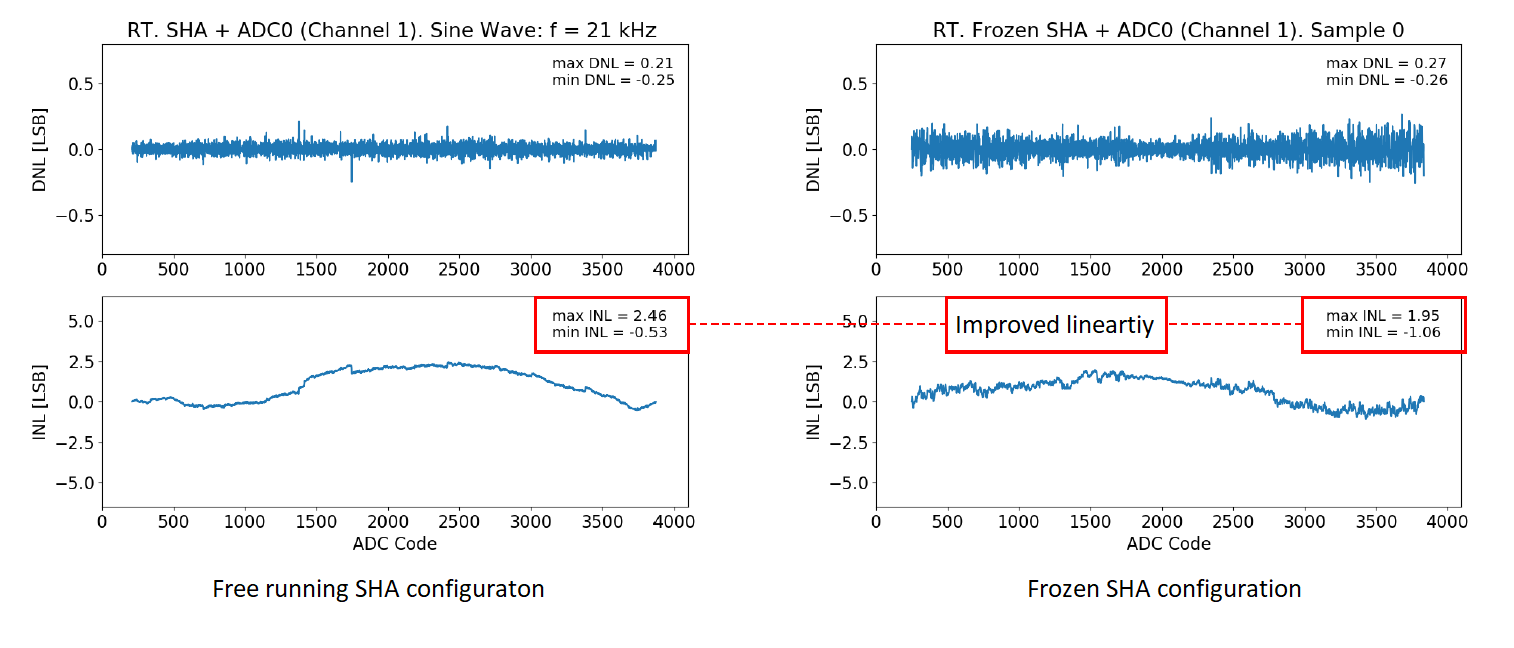
\includegraphics[width=1\linewidth]{figures/prakash_fig/linearity_rt_free_frozen.png}
  \caption{Linearity comparison of the ADC with single ended input in free running SHA and frozen SHA mode at room temperature}
  \label{fig:linearity_rt_free_frozen}
\end{figure}

While running more experiments in free running SHA configuration at LN2 temperature, spikes were observed in the DNL plots, these spikes does not appear in frozen SHA configuration. Figure \ref{fig:linearity_free_frozen} show the difference in linearity for free running SHA mode and frozen SHA mode at LN2 temperature and the 10 most extreme values are labeled in the plots. We believe MUX's are the main cause of spikes, it is very difficult to simulate MUX's effects on ADC linearity. We are still in the process of understanding and proving the root cause for linearity degradation and appearance of spikes in simulations. To fix this, we will redesign the MUX's to be faster. 
%A possible explanation for this is the ON resistance of the switches (MUX) is significantly larger at cold than at room temperature. Redesigning the MUX to be faster will solve this problem. 
\begin{figure}[h!]
\centering
  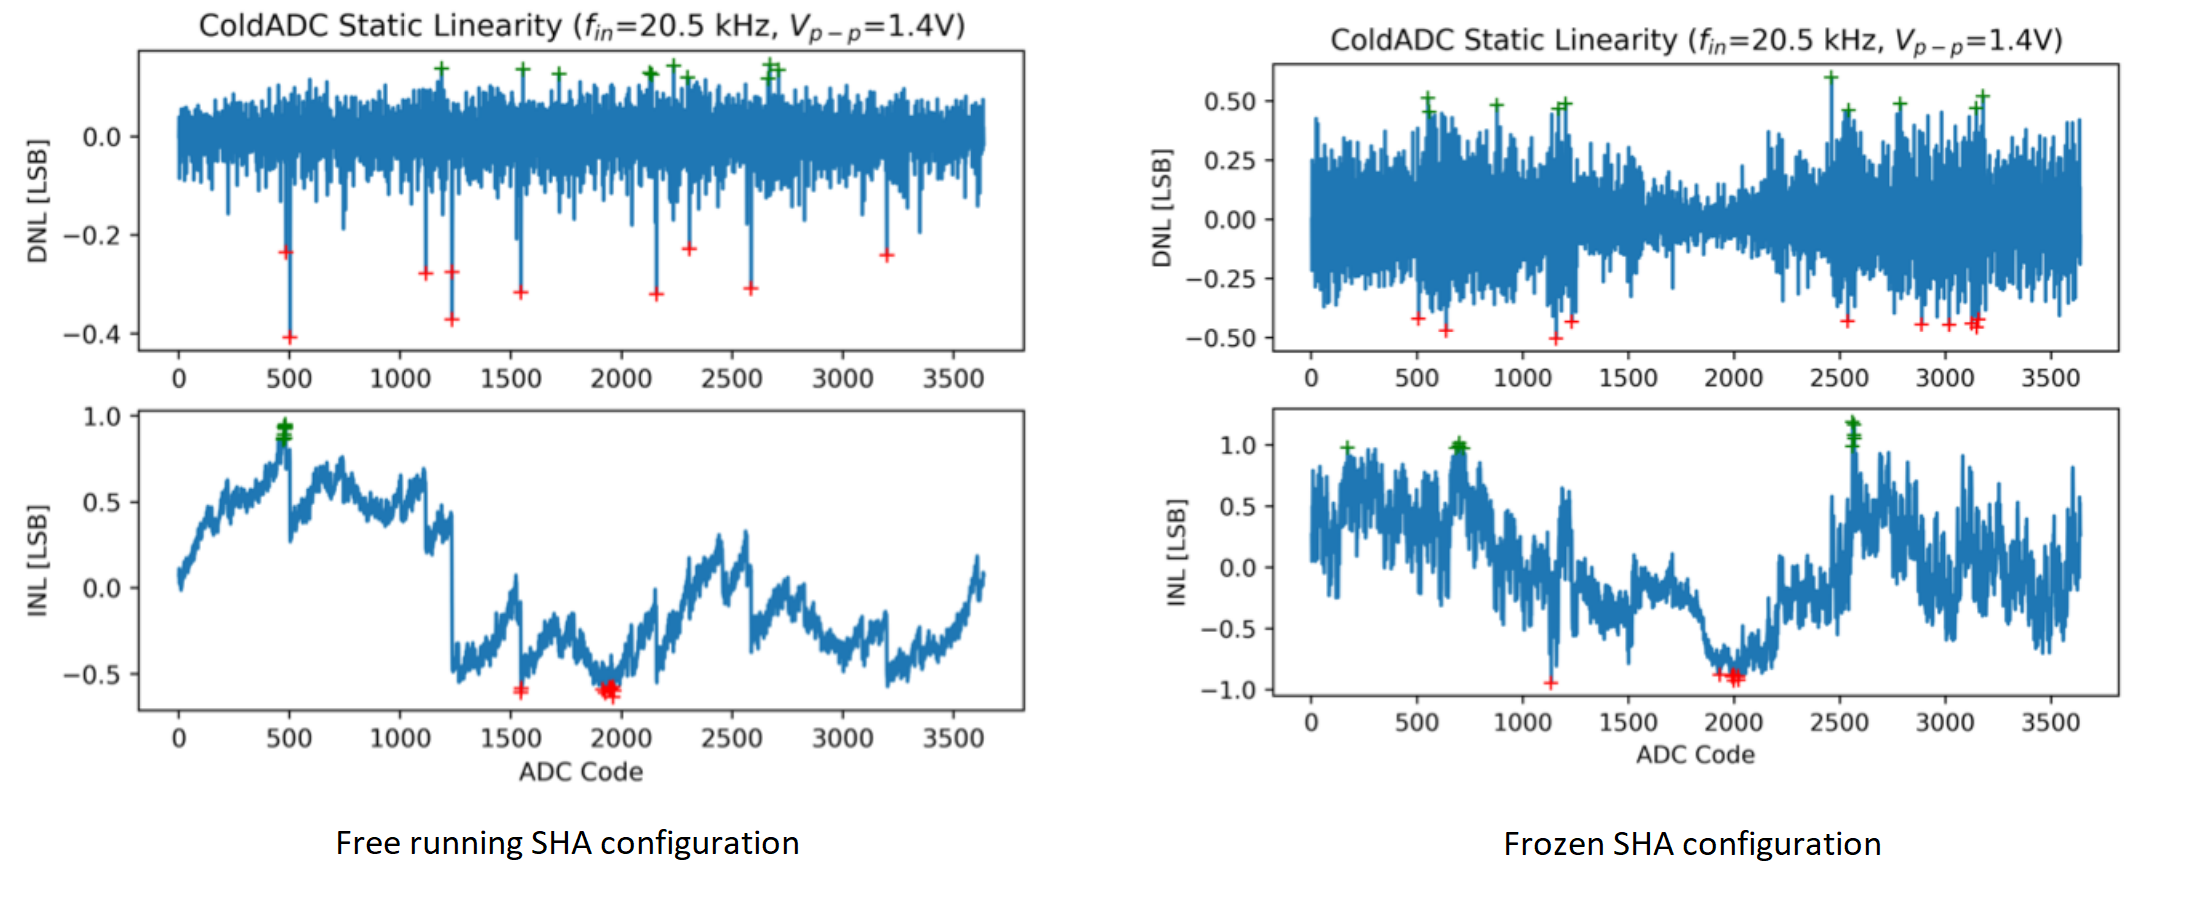
\includegraphics[width=1\linewidth]{figures/prakash_fig/linearity_free_frozen.png}
  \caption{Linearity comparison of the ADC with single ended input in free running SHA and frozen SHA mode at LN2 temperature}
  \label{fig:linearity_free_frozen}
\end{figure}